% %%%%%%%%%%%%%%%%%%%%%%%%%%%%%%%%%%%%%%%%%%%%%%%%%%%%%%%%%%%%%%%%%%%%%%
% The State:
% %%%%%%%%%%%%%%%%%%%%%%%%%%%%%%%%%%%%%%%%%%%%%%%%%%%%%%%%%%%%%%%%%%%%%%
\fancychapter{State of the art}
\label{cap:state}

This chapter will go over the several subject that need to be known in order to understand the thesis.

Math is the best way to universally describe all scientific models. For this reason, this chapter, and the thesis as whole, will contains equations.

It seems only logical to define all the tools that are going to be used in the thesis.

\begin{itemize}
  \item Vectors are displayed as $\overrightarrow{v}$ and are considered to be vertical matrixes, matrixes of size ($1\times n$) for vector of size $n$.
  \item $\overrightarrow{1}$ represent a vector that only contains ones of variable size.
  \item $\odot$ is used for the Hadamart product, that is the point wise multiplication of each element of the matrixes
  \item $\cdot$ is used in two cases :
    \begin{itemize}
      \item When used with scalars, it is the product of those scalars.
      \item When used with matrixes, it is the matrix product
    \end{itemize}
  \item $+$ is also used in two cases :
    \begin{itemize}
      \item When used with scalars, it is the sum of those scalars.
      \item When used with vectors (column matrixes), it is the point wise sum, basically adding each element to each other. The result is a vector of the same size.
    \end{itemize}
\end{itemize}


\section{\acl{AI}}\label{sec:ai}

\acf{AI} is very popular, and is getting more attention, being used as selling point by lots of services, the word is thrown around so much that it lost its meaning. So what are \acp{AI} exactly.

\ac{AI} is defined as theories and stragies used to simulate human intelligence, in other words, a computer or software that can take a decision by itself based on previously set rules. The definition is very wide and have lots of ways to be implemented.

The most commonly used type of \ac{AI} is machine learning, which consists of teaching the software to make decision. It is defined as the use and development of computer systems that are able to learn and adapt without following explicit instructions, by using algorithms and statistical models to analyse and draw inferences from patterns in data.

\subsection{Machine learning}

In the last 10 years, the research concerning machine learning has considerably increased.

%TODO add superbe diagram
\begin{figure}[H]
  \centering
  \includesvg[width=.96\textwidth]{ml.svg}
  \caption{Machine learning and all its substypes}
  \label{fig:ml}
\end{figure}

% For the State of the art

\ac{AI} is wide topic, usually when we talk about \acp{AI}, we refer to the most common type, Machine Learning. Especially, a sub part of Machine Learning called Deep Learning. Deep Learning has seen a surge in research the last decade, which lead to great advancement in this field and the numerous \ac{AI} tools that popped up in the last years.
Deep Learning works using what is called \acp{NN}.

Those \acp{NN} require matrix multiplication. This kind of operation is very time and energy consuming to run on a classic computer. There are options to better run those operations. GPUs can be better suited than a CPU for a \ac{NN} application as it is made for 3D graphics that also mainly use Matrix Multiplication. Other specialized hardware such as FPGAs and ASICs can improve both execution time and energy consumption. All those are digital computers, using analog computing could highly improve speed, power consumption and even smaller chip area. All this using a memristive crossbar array \cite{Xbar}. An analog computer
The point of this thesis is to lay out the ground work to create a LSTM capable chip to use in embedded systems. It could be used detection and prediction of any kind of sequential events.
Using those memristors \cite{TheoMemristor}, which work like resistance with a memory component to them, that means that they can be set to a desired value.

\section{Neural Networks}\label{sec:nn}

\acfp{NN} are a network of several layers of artificial neurons. Figure \ref{fig:snn}, shows a simple representation of a \ac{NN}, the artificial neurons are the represented by the colored circles. On figure \ref{fig:snn} each arrow represent a synapse.

\begin{figure}[h!]
  \centering
  \includesvg[height=8cm]{NN_explained.svg}
  \caption{Simple \acl{NN}}
  \label{fig:snn}
\end{figure}



They are several layers to a \ac{NN} :
\begin{itemize}
  \item Input layer : This layer is simply the different inputs.
  \item Hidden layer : This layer can be (and usually is) wider than the one in figure \ref{fig:snn}, it is there to add more layers and thus more precision to the result
  \item Output layer : This layer is where you can find the result from the \ac{NN}.
\end{itemize}

In a computational \ac{NN}, synapses are represented by weights. Those weights are to be multiplied by the last neuron and then added to each other to produce the next stage. Using the names defined in figure \ref{fig:snn}, the equation linking each layer is the following matrix multiplication :
\begin{equation}
  \begin{bmatrix}
    H1\\ H2\\ H3\\ H4\\
  \end{bmatrix}
  =
  \begin{bmatrix}
    W1,1 & W1,2 & W1,3\\
    W2,1 & W2,2 & W2,3\\
    W3,1 & W3,2 & W3,3\\
    W4,1 & W4,2 & W4,3\\
  \end{bmatrix}
  \cdot
  \begin{bmatrix}
    I1\\ I2\\ I3\\
  \end{bmatrix}
\end{equation}

And it works the same way to go to the next layer.


Those matrix multiplication are very power-hungry and their computation time scales up with the size of the \ac{NN} using classical computing.

Analog computation enables those same calculations almost instantly and being far more power-efficient. This can be done using the physical properties of electrical devices.
We want to reproduce one of those neural network using electrical circuits to perform the same computation that a computer would in much faster manner.
Using \hyperref[subsec:memristors]{memristors} as weights. This removes the need to copy the weights from the main memory

\section{\acs{RNN}}\label{sec:rnn}

\acp{RNN} are, as the name suggests, a type of \ac{NN} using recurrent connections. They are a \ac{NN} with at least one cycle within the structure, where outputs of the previous run is used the next one. Those feedback connections are what differenciates it from feedforward \ac{NN}.

This type of \ac{NN} is used when dealing with an unknown amount of inputs. Especially useful when treating time series \cite{rnn}. Example of \acp{RNN} uses are speech recognition, automatic language translation \cite{gru} and shape recognition, especially for handwriting recognition.

Traditionnal \ac{RNN} have the ability to model sequential events by propagating through time, for example forward and backward propagation. This is achieved by connecting these sequential events with the hidden state like in \cref{eq:rnn}.

\begin{equation}\label{eq:rnn}
  \overrightarrow{h_t}=f(\overrightarrow{x_t},\overrightarrow{h_{t-1}})
\end{equation}

The hidden state ($\overrightarrow{h_t}$) carries all the past informations for the next time step. It also serves as the output of the \ac{RNN}.

They are trained the same way \ac{NN} are, measuring the error, backpropagte and adjust the weights accordingly.

\subsection{Simple \ac{RNN}}

The simple \ac{RNN} works just like a \ac{tanh} activated feedforward \ac{NN} with a feedback connection.

\Cref{eq:srnn} shows the equation that the simple \ac{RNN} runs at every time step.

\begin{equation}\label{eq:srnn}
  \overrightarrow{h_t}=tanh([\overrightarrow{x_t},\overrightarrow{h_{t-1}}]\cdot w + b)
\end{equation}

Where $t\in\mathbb{N}^*$ is the time index, $w$ the weight matrix, $b$ the bias matrix, $\overrightarrow{x_t}$ the input vector and $\overrightarrow{h_{t}}$ the hidden state of the \ac{RNN}.

\subsection{Vanishing gradient problem}

The Vanishing gradient problem is a problem that comes when dealing with time depedent data \cite{vanishGrad}. When big amount of time depedent data is fed to the \ac{RNN}, the weights can't be updated properly. The older the data, the lower it will impact how much the weight must change. Rendering the old input data almost useless. Simple \acp{RNN} must be used with relatively short time series.

Some \acp{RNN} were designed around this issue. This is the case of the \ac{LSTM} and \ac{GRU} which were created with internal mechanisms to regulate the flow of information and gradients.

\section{LSTM}\label{sec:lstm}
\acp{LSTM} are a type of \ac{NN} used to analyze sequence of data. They are capable of predict data based of the previous results. \acp{LSTM} are part of \acp{RNN}. \acp{RNN} are different than feedfoward \acl{NN} because of their feedback connections. Meaning that the results from the last time step have an impact on the next time step.

\acp{LSTM} were born from the vanishing/exploding gradient problem. Traditionnal \ac{RNN} have the ability to model sequential events by propagating through time, for example forward and backward propagation. This is achieved by connecting these sequential events with the hidden state:
$$h_t=f(h_{t-1},x_t)$$
The hidden state $h_t$ carries all the past informations for the next time step.
Even though \acp{RNN} work very well, they are subject to the vanishing/exploding gradient problem. This issue occurs when too many time steps are chained.

\acp{LSTM} alleviate this issue by adding a cell state, this state gives it the ability to choose what input is important and which one isn't, thus giving it a long term memory. This ability gave the uncommon name of \acl{LSTM} as it has both long and short term memory. This what gives \acp{LSTM} their use for sequence data. They can analyze the data and keep the information from the last time step to make a better decision afterwards. The most comprehensible example is considering a sentence. (TODO : find example)

An \ac{LSTM} is more complicated than just a simple feedforward \acl{NN}, they have several gates, which are all technically a \ac{NN} themselves. There is also a cell state which job is to hold a value for the next step.

\begin{figure}[H]
  \centering
  \includesvg[width=\textwidth]{lstm/lstmCell.svg}
  \caption{LSTM Cell}
  \label{fig:lstmCell}
\end{figure}

Figure \ref{fig:lstmCell} shows the complexity of the \ac{LSTM} architecture. In an \ac{LSTM}, each gate is a different \ac{NN} and then activated with either a tanh or a sigmoid activation function. Each input to the cell is a vector.
Those vector are of varying sizes depending on several factors. For example, both $h_t$ and $c_t$ are of the same size as the number of hidden state (sometimes refered to as cell state) for any $t\geq 0$.
The input vector ($x_t$) is of size of the sample we want to feed for each time step.

\subsection{Equations}

The equations of an LSTM are quite unusual.
Let's start with the more classic gate equations. They are the ones that behave like the more classic \ac{NN}.
The input (equation \ref{eq:inputG}), forget (equation \ref{eq:forgetG}) and ouput (equation \ref{eq:ouputG}) gates are described below.

\begin{equation}\label{eq:inputG}
  i_t=\sigma (w_i\cdot[x_{t_1},h_{t-1}] + b_i)
\end{equation}
\begin{equation}\label{eq:forgetG}
  f_t=\sigma (w_f\cdot[x_{t_1},h_{t-1}] + b_f)
\end{equation}
\begin{equation}\label{eq:ouputG}
  o_t=\sigma (w_o\cdot[x_{t_1},h_{t-1}] + b_o)
\end{equation}

Where ($w_i$,$b_i$), ($w_f$,$b_f$) and ($w_o$,$b_o$) are the pair of weights and biases for the input, forget and ouput gates respectively. $x_t$ is the input vector and $h_t$ is the hidden state vector.

For the next equation describes the candidate cell state (equation \ref{eq:candCell}), that will next become the cell state (equation \ref{eq:cellS}).

\begin{equation}\label{eq:candCell}
  \tilde{c}_t=tanh(w_c\cdot[x_{t-1},h_{t-1}] + b_c)
\end{equation}
\begin{equation}\label{eq:cellS}
  c_t=f_t\cdot c_{t-1} + i_t \cdot \tilde{c}_t
\end{equation}

Where $w_c$ and $b_c$ are the weights and bias for the candidate cell state.

The final step of the \ac{LSTM} is to compute the hidden state (equation \ref{eq:hiddenS}).
\begin{equation}\label{eq:hiddenS}
  h_t=o_t\cdot tanh(c_t)
\end{equation}

We set $x_0$ as the first input and define $h_0$ as a zero only vector.

\subsection{Usage}

\section{\acs{GRU}}
The \acf{GRU} is another type of \ac{RNN}. It is also known to reduce the effect of the vanishing gradient problem. It was first introduced to improve translation techniques \cite{gru}.

The \ac{GRU} is very often compared to the \ac{LSTM}, it is sometimes assimilated as a type of \ac{LSTM} \cite{nbLSTM}. Their performance was found to be very similar in most situations, making those two types of \acp{RNN} coexistant in the modern machine learning world.

There are two versions of the \ac{GRU}, both are found on the internet, they are known as the encoder and decoder version \cite{gru}. They were originally designed to encode the message to translate and then decode in the translation. PyTorch only supports the decoder version \cite{gruPyTorch}, while the keras library supports both \cite{gruKeras} chosen by changing an argument.

\subsection{Encoder \ac{GRU}}

The encoder \ac{GRU} is the version of the \ac{GRU} most widely described on the internet. It contains an update gate (\cref{eq:updateG}), a reset gate (\cref{eq:resetG}), a candidate activation gate (\cref{eq:candActivG}). The hidden state is then computed (\cref{eq:gruHidG}) using the previous results.

\begin{equation}\label{eq:updateG}
  \overrightarrow{z_t}=\sigma ([\overrightarrow{x_t},\overrightarrow{h_{t-1}}] \cdot w_z + \overrightarrow{b_z})
\end{equation}
\begin{equation}\label{eq:resetG}
  \overrightarrow{r_t}=\sigma ([\overrightarrow{x_t},\overrightarrow{h_{t-1}}] \cdot w_r + \overrightarrow{b_r})
\end{equation}
\begin{equation}\label{eq:candActivG}
  \overrightarrow{\hat{h_t}}=tanh(\overrightarrow{x_t}\cdot w_{hx}+(\overrightarrow{r_t}\odot\overrightarrow{h_{t-1}}) \cdot w_{hh} + \overrightarrow{b_h})
\end{equation}
\begin{equation}\label{eq:gruHidG}
  \overrightarrow{h_t}=(\overrightarrow{1}-\overrightarrow{z_t})\odot \overrightarrow{h_{t-1}} + \overrightarrow{z_t}\odot \overrightarrow{\hat{h_t}}
\end{equation}

Where ($w_z$,$\overrightarrow{b_z}$), ($w_r$,$\overrightarrow{b_r}$),($w_{hx}$,$w_{hh}$,$\overrightarrow{b_h}$) are the weights matrixes and bias vectors for the update, reset and candidate activation gates respectively.

Sometimes the \cref{eq:gruHidG} can be found in another form (\cref{eq:gruHidG1})\cite{gruPyTorch}. This, however, has no impact on the final results, it means the weights are going to be trained differently for the update gate.

\begin{equation}\label{eq:gruHidG1}
  \overrightarrow{h_t}=\overrightarrow{z_t}\odot \overrightarrow{h_{t-1}} + (\overrightarrow{1}-\overrightarrow{z_t})\odot \overrightarrow{\hat{h_t}}
\end{equation}

\subsection{Decoder \ac{GRU}}

The decoder \ac{GRU}, while being less described, is the version used in pyTorch, which is getting very popular.

The candidate activation gate (\cref{eq:candActivG1}) is the only difference from the encoder \ac{GRU}.

\begin{equation}\label{eq:candActivG1}
  \overrightarrow{\hat{h_t}}=tanh(\overrightarrow{x_t}\cdot w_{hx}+ \overrightarrow{b_{hx}}+\overrightarrow{r_t}\odot[\overrightarrow{h_{t-1}} \cdot w_{hh} + \overrightarrow{b_{hh}}])
\end{equation}

\subsection{Similarities with \ac{LSTM}}

The \ac{CIFG} \ac{LSTM} or more commonly known as \ac{GRU}. \cite{gru,gruKeras,gruPyTorch} As it's name implies, \acl{CIFG}, links the input and forget gates as such, $f_t=1-i_t$. Other differences are :
\begin{itemize}
  \item No peepholes and output activation function.
  \item Combined hidden state and cell state.
  \item The candidate cell state is point wise multiplied with the output gate before the activation function.
\end{itemize}

This is clearer with the math equations :
\begin{equation}\label{eq:cellGGRU}
  \tilde{c}_t = tanh(w_{cx}\cdot x_t + w_{ch}\cdot(o_t \odot h_{t-1}) + b_c)
\end{equation}
\begin{equation}\label{eq:hiddenGRU}
  h_t=(1-i_t)\cdot h_{t-1} + i_t \cdot \tilde{c}_t
\end{equation}

\section{Memristors}
\label{sec:memristors}

Memristors are the lesser known fourth fundamental passive component of electronics, among resistors, capacitors and inductor.
It was first theorized in 1971 by L. Chua from UC Berkeley, in \cite{TheoMemristor}. The name comes from the blend of \textit{memory} and \textit{resistance}.
The theory behind this component was extracted from a missing component to link the four fundamental circuit variables, voltage ($v$), charge ($q$), current ($i$) and flux ($\phi$). \Cref{fig:fundComp} shows the four fundamental variables are on each side of the square, with the ones on opposite sides being linked by the following equations :
\begin{equation}
  d\phi = v\cdot dt
\end{equation}

\begin{equation}
  dq = i\cdot dt
\end{equation}

Resistors, capacitors and inductors were already very established and well known component, so it was theorized that a fourth device should then exists to physically link flux ($\phi$) and charge ($q$).  The flux in this case is not a magnetic flux and is defined as such : $ d\phi=v\cdot dt \Rightarrow \phi =  \int v \,dt  $.\\
The component stayed theoretical until 2008 when it's been implemented in a physical device for the first time \cite{memristorFab}. It took 37 years to have an actual working device.\\
There is then an extention of this theoretical device to another, the memristive device. It was theorized in 1976 by L. Chua and S. M. Kang \cite{memrestiveDev}. The difference between the memristor and the memristive device is its internal behavior. Memristive device are commonly referred to as memristor as well.

\begin{figure}[H]
  \centering
  \includesvg[width=0.55\textwidth]{memristor/memristor}
  \caption{Fundamental passive components}
  \label{fig:fundComp}
\end{figure}

\subsection{Equations}
A memristor links the flux ($\phi$) and charge ($q$) and creates the memristance.
This memristance is defined with the following equation :
\begin{equation}
  M(q)=\frac{d\phi}{dq}
\end{equation}
It can be compared with the other fundamental components like resistor ($R(i)=\frac{dv}{di}$), capacitor ($\frac{1}{C(q)}=\frac{dv}{dq}$) and inductor ($L(i)=\frac{d\phi}{di}$).
We can then extract a more useful equation in an actual circuit :
\begin{equation}
  v(t)=M(q(t))\cdot i(t)
\end{equation}
Similarly, a memductance can be defined as such :
\begin{equation}
  W(\phi)=\frac{dq}{d\phi}
\end{equation}
A memristive device is slightly differently defined, it still uses a memristance, but here the memristance also depends on an internal state called $x$. This gives us this equation :
\begin{equation}
  v(t)=M(x,i)\cdot i(t)
\end{equation}
The internal state ($x$) is not linked to flux or charge in the case of a memristive device.\\
Once again, we can also define the memristive device using a memductance :
\begin{equation}
  i(t)=W(x,v)\cdot v(t)
\end{equation}
In all of the previous equations, $v$ is the voltage in Volt ($V$), $i$ is the current in Ampere ($A$), $\phi$ is the flux in Weber ($Wb$), $q$ is the charge in Coulomb ($C$), $M$ is the memristance in Ohm ($\Omega$) and $W$ is the memductance in Siesmens ($S$ or $\Omega^{-1}$).

\subsection{Behavior}

A memristor is defined as a non-linear two-terminal fundamental electrical component. It behaves as a resistance with memory (hence its name), meaning that it changes its resistance based on how much charge went through it. This enables us to manipulate the resistance of the component.
The huge benefit of memristors its ability to retain its internal resistance, the device can left without power for a long period of time (retention time of minimum 10 years according to \cite{memRetention}). When the device is powered backup, it will have the same resistance it had before.

Memristive devices have a similar behavior, the memristive device's resistance will change depending on the internal state ($x$). That internal state changes based on how much and how long voltage signals or currents are applied to the memristive device.

\subsection{Usage}
The main research for memristor usage is using them as ReRAM. The idea behind ReRAM is to use memristors as Non-Volatile memory. It uses two states of the device with known resistances ($R_{on}$ and $R_{off}$), giving it binary property. Reading the memory simply requires setting a voltage and reading the output current. It is better than current solutions (HDD, SSD) as it has a much lower latency. It is better than traditionnal DRAM because it keeps the information even when turned off. This makes ReRAM a good replacement for both RAM and HDDs/SSDs, thus eliminating Von Neumann bottleneck due to the Von Neumann architecture that is used in all modern computers.

They can also be used to set a resistance to be able to perform analog multiplication. Setting them in a crossbar array makes them a very strong candidate to be used in neuromorphic computing.

\section{Memristors Crossbar Array}\label{sec:crossbar}

Setting memristors in a crossbar array allows to perform analog \ac{VMM} also called Multiply and Accumulate. This circuit works great for this use as all the computation is done almost instantly and using physics laws. Figure \ref{fig:crossbar} shows what a typical crossbar array looks like.

\begin{figure}[H]
  \centering
  \subfloat[Schematics]{\includesvg[width=.45\linewidth]{crossbar/crossbar}}%\qquad
  \hfill
  \subfloat[3 dimensional representation]{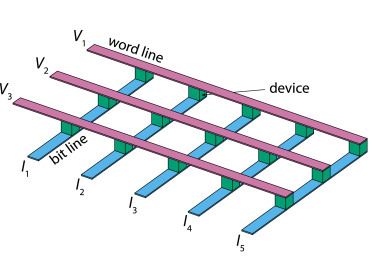
\includegraphics[width=.45\linewidth]{crossbar/crossbar3D.jpg}}\\
  \caption{Memristor crossbar array}
  \label{fig:crossbar}
\end{figure}

It uses physical properties of electrical systems to perform analog computing. Lets use the circuit node in figure \ref{fig:crossNode} to explain the theory behind the memristor crossbar array.
\begin{figure}[H]
  \centering
  \includesvg[height=3.5cm]{crossbar/node}
  %\def\svgheigth{3.5cm}
  %\input{crossbar/node.pdf_tex}
  \caption{Memristor crossbar node of the $i^{th}$ line and $j^{th}$ column}
  \label{fig:crossNode}
\end{figure}

First of all, a voltage is applied on the $i^{th}$ line, because every column is virtually grounded, the voltage applied to the memristor, of a set resistance $R_i$, is $V_i$. As such and using Ohm's law, we know the the current flowing into the memristor ($I_{mem}$) is bound by the following equation :

\begin{equation}
  V_i = R\cdot I_{mem} \Rightarrow I_{mem} = V_i\cdot (\frac{1}{R})=I_{mem} = V_i\cdot\sigma_i
\end{equation}
With $\sigma_i$ being the conductance of memristor, defined as $\sigma_i=\frac{1}{R_i}$.

This line then joins the column where a current of $I_{i,j-1}$ is flowing, then according to kirchhoff's current law the resulting current is :
\begin{equation}
  I_{j,i} = I_{j,i-1}+I_{mem} = I_{j,i-1} + V_i\cdot\sigma_i
\end{equation}
By applying this process to the whole system we find that the current as the bottom of one column is :
\begin{equation}
  I_1=\sigma_1\cdot V_1 + \sigma_2\cdot V_2 + \sigma_3\cdot V_3
\end{equation}
With $\sigma_1$, $\sigma_2$ and $\sigma_3$ being the conductance of the 3 memristors in the first column.

This analog circuit removes the need to copy data from a main memory as the memristors themselves hold the value and the weights are then stored where the computation happens.%TODO elaborate

\section{Memristor's model}\label{sec:model}
They are several ways to model a memristor (TODO : cite).

One of them, works by applying voltage pulse to the device. The device then change it's internal resistance based on how far from the stable point (usually the initial resistance) it is.
TODO


\cleardoublepage
